\documentclass{article}
\usepackage[utf8]{inputenc}
\usepackage[spanish]{babel}
\usepackage{listings}
\usepackage{graphicx}
\graphicspath{ {images/} }
\usepackage{cite}

\begin{document}

\begin{titlepage}
    \begin{center}
        \vspace*{1cm}
            
        \Huge
        \textbf{Proyecto Final}
            
        \vspace{0.5cm}
        \LARGE
        Los primeros pasos
            
        \vspace{1.5cm}
            
        \textbf{Integrantes\\}
        \textbf{Juan Diego Cabrera Moncada}
            
        \vfill
            
        \vspace{0.8cm}
            
        \Large
        Departamento de Ingeniería Electrónica y Telecomunicaciones\\
        Universidad de Antioquia\\
        Medellín\\
        Marzo de 2021
            
    \end{center}
\end{titlepage}

\tableofcontents
\newpage
\section{Sección introductoria}\label{intro}
El videojuego que deseo desarrollar es del género de puzzle, de modo que la idea general del juego es plantear 5 niveles, los cuales tienen diferente dificultad, y cada uno cuenta con su propia escena. El juego está planteado para poner a prueba el analisis del jugador más que su habilidad para derrotar enemigos. De modo que el principal objetivo es ofrecer al jugador un problema complejo de resolver (No pueda ser resuelto de forma inmediata) \cite{Puzzle}. Este juego es de tipo multijugador cooperativo, específicamente para 2 jugadores. Cabe destacar que cada objeto mencionado, en el código implementado, corresponde a una clase diferente. Así, todos los objetos mencionados en la sección de Personajes, requieren de la creación de una clase propia (Los objetos a los que se puede vincular el jugador, mencionados en la subsección Personajes Principales, son los mismos que los mencionados en la sección Objetos).
\section{Desarrollo del juego}
Para ganar el nivel, los jugadores debe dirigir sus personajes hacia el objeto que representa el término del nivel, es decir, una vez entran en contacto con dicho objeto, los jugadores pueden avanzar al siguiente nivel dado caso que se trate de los primeros 4 niveles, o terminar el juego si se trata del último nivel. Los jugadores cuentan con 3 vidas, si alguno de los 2 entra en contacto con un objeto que pueda restar una de ellas, se reinicia automáticamente el nivel y se descuenta una de sus vidas, una vez este contador llegue a cero, se redirecciona a los jugadores al primer nivel. El punto de partida en el cual inician ambos personajes principales es el mismo para todas las escenas; no obstante, cada escena cuenta con sus propios puntos para ubicar el resto de objetos que la conforman. Los jugadores deben tener en cuenta que su movimiento está restringido sólo al desplazamiento a través de los cables que haya en la escena.
\section{Escenas}
Previamente a proceder con la descripción de cada escena, hago énfasis en que cada escena corresponde a uno de los niveles del juego.
\subsection{Primera escena}

\subsection{Segunda escena}

\subsection{Tercera escena}

\section{Personajes}
\subsection{Personajes principales}
Los personajes principales son objetos tipo luces de electricidad que son capaces de proporcionar electricidad a diferentes objetos, para poder vincularse a un objeto deben estar inmediatamente próximos a ellos, y para vincularse lo deben hacer oprimiendo una tecla predeterminada, y para desvincularse se usa la misma tecla. Asimismo se tiene pensado que las interacciones con los diferentes dispositivos al estar vinculados a ellos se haga con las mismas teclas que el jugador usa para el movimiento del personaje, además de añadir una tecla de activación y desactivación de interacción. De esta manera, se tiene pensado que los dispositivos a los cuales se puede vincular sean los siguientes:
    - Cañón: Al vincularse con un cañon, hace que éste se ilumine y permita realizar un disparo a la vez de una bola de cañón con una cantidad limitada de tiros en forma de un tiro parabólico. Dependiendo de cuántos jugadores se vinculen a un cañón en específico, éste permite hacer un tiro de menos o de más potencia con la tecla de interacción. Cabe destacar que la bola de cañón es destruida instantáneamente al entrar en contacto con un objeto tipo muro.
    - Foco de luz: Esta forma permite al jugador proyectar un haz de luz en una dirección específica una vez vinculado, cuando se activa la tecla de interacción. Dicho haz de luz tiene la capacidad de hacer un efecto de reflexión total, reflexión difusa o un efecto de refracción dependiendo de los objetos en los que se proyecte. Sólo un jugador se puede vincular a un foco de luz.
    - Bombilla: Cuando ambos jugadores se vinculan a ella con la suficiente energía, se les permite avanzar al siguiente nivel. Así, como mínimo uno de los jugadores debe estar en un tamaño medio (Hay tamaño grande, medio y pequeño) para poder avanzar de nivel.
    - Cargador: Cuando uno o dos jugadores se vinculan a un cargador, dependiendo de cómo fue previamente configurado, éste provoca la activación de un mecanismo en específico (Explicado en el apartado Objetos).
\subsection{Enemigos}
Se tiene planteado así los siguientes enemigos (Los enemigos también se plantean como objetos del juego):
    - Resistor circular: Este enemigo es estático. Las primeras 2 veces que entran en contacto con uno de los jugadores reducen su tamaño, indicando que poseen una menor cantidad de electricidad, y la tercera vez le quitan una vida a los jugadores, haciendo que ambos regresen a su posición inicial. Hay que aclarar que si el jugador con el que chocó choca nuevamente con el mismo resistor, éste le devuelve el tamaño que le había quitado. Su imagen es la siguiente:
    - Sierra circular: Son usados como obstáculos para el espacio dentro del cual se espera que los jugadores puedan disparar sus bolas de cañón. Cuando una bola de cañón entra en contacto con ellos, la bola es destruida instantáneamente. Las sierras circulares pueden ser estáticas, experimentar un movimiento pendular o un movimiento circular uniforme. La diferencia entre una sierra y un muro corresponde a que los muros sólo representan los límites del espacio mientras las sierras pueden estar en cualquier posición del espacio distinta de los límites del mismo.
\section{Objetos}
\subsection{Cañón}
Más de un jugador puede vincularse a un cañón, y éste se encarga de generar objetos tipo bola de cañón en la dirección especificada por el jugador.
\subsection{Bola de cañón}
Es un objeto generado por el jugador al oprimir la tecla de disparo. No obstante, solo se puede generar un objeto tipo cañón a la vez para mostrar en escena. Este objeto experimenta un efecto de movimiento parabólico, con su magnitud y dirección iniciales del movimiento indicadas por el jugador.
\subsection{Foco de luz}
Cualquier jugador puede vincularse a este objeto, pero sólo uno a la vez. Una vez vinculado, emite un objeto tipo haz de luz, el cual cambia su dirección dependiendo de las teclas oprimidas por el jugador usando el objeto tipo foco de luz.
\subsection{Haz de luz}
Est objeto se propaga en una dirección determinada, de modo que al interactuar con un cristal, su dirección llega hasta al cristal y después se altera siguiendo la lógica de un efecto de reflexión total. Al interactuar con un muro, una plataforma móvil o una sierra circular, experimenta un efecto de reflexión difusa. Al interactuar con un panel solar, activa la función del mismo. No interactúa con el resto de objetos.
\subsection{Fondo}
Este objeto representa aquellos puntos de la escena en los cuales no se encuentra ningún objeto con el cual el jugador pueda interactuar. Un jugador no puede desplazarse por el espacio que ocupa el fondo a menos de que hayan cables que permitan su movimiento a través de él. 
\subsection{Muro}
Sirven para eliminar las bolas de cañón una vez éstas entran en contacto con el muro. Asimismo, el haz de luz se propaga mostrando su trayecto hasta antes de entrar en contacto con un muro.
\subsection{Cristal}
Cuando un cristal entra en contacto con un haz de luz, el haz de luz experimenta un efecto de reflexión total.
\subsection{Panel solar}
Cuando un panel solar entra en contacto con un haz de luz, éste se carga activando una plataforma móvil.
\subsection{Cargador}
Cuando los jugadores se vinculan a un cargador, éste puede que active una plataforma móvil, conecte o desconecte una serie de cables. Más de un jugador puede vincularse al mismo cargador.
\subsection{Plataforma móvil}
Este objeto se puede desplazar una distancia predefinida y es capaz tanto de bloquear un haz de luz como de destruir una bola de cañón. No obstante, puede actuar de distintas formas: 
En la primera de ellas, la plataforma móvil sólo se desplaza de su posición inicial cuando es cargada por acción del vínculo de uno de los jugadores con un objeto específico tipo cargador o panel solar, para el caso del objeto tipo cargador, la plataforma móvil se desplaza una distancia diferente dependiendo de la cantidad de jugadores vinculados al cargador. Cabe destacar que el jugador no debe mantenerse vinculado al cargador para que la plataforma se mantenga en su posición final o para que continue desplazándose.
En la segunda de ellas, lo hace de forma automática, desplazando de un punto a otro en un eje vertical u horizontal determinado.
\subsection{Cables}
Son el único medio posible por el cual se pueden desplazar los jugadores. Así, donde no hayan cables, los jugadores no pueden acceder a dicho punto.
\subsection{Bombilla}
Permite avanzar al siguiente nivel, pero para ello, ambos jugadores deben llegar a la bombilla para proporcionarle la suficiente energía para que ésta se encienda y puedan pasar a la siguiente fase.
\section{Planificación de actividades}
La planificación de las actividades a desarrollar para poder completar el juego se resumen en el siguiente cronograma.
\begin{figure}[h]
    \centering
    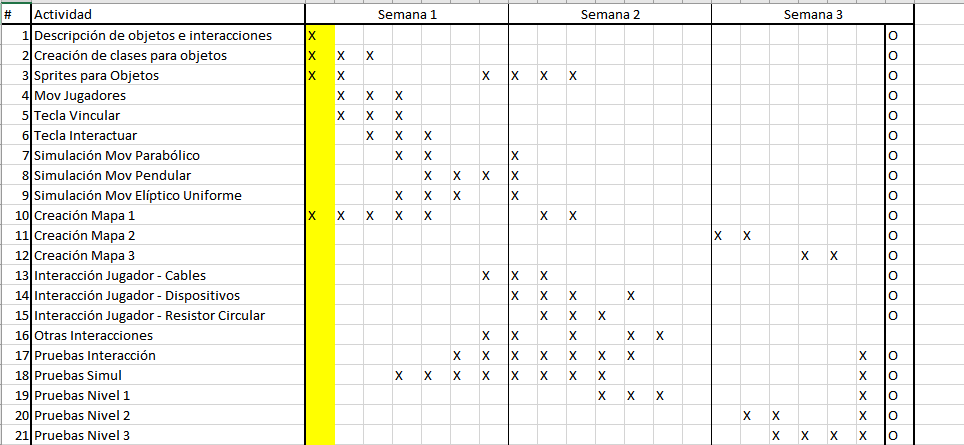
\includegraphics[width=14cm]{Crono_1.png}
    \caption{Cronograma parte 1}
    \label{fig:crono_1}
\end{figure}
\begin{figure}[h]
    \centering
    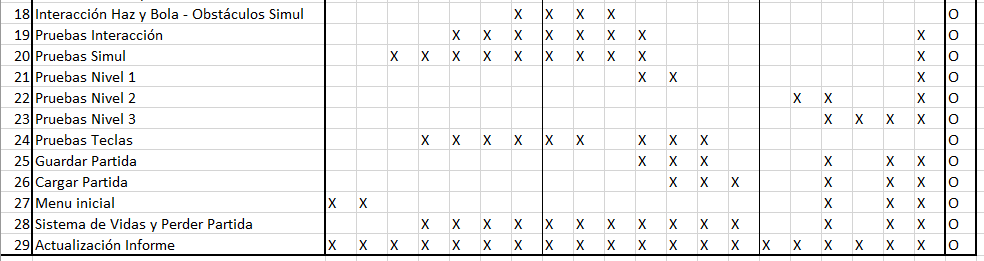
\includegraphics[width=14cm]{Crono_2.png}
    \caption{Cronograma parte 2}
    \label{fig:crono_2}
\end{figure}
\bibliographystyle{IEEEtran}
\bibliography{references}

\end{document}
